\chapter{Die Skelettierung}
\label{ch:Skelettierung}
\Autor{Sandra Schröder}\\\\
Unter einem Skelett kann man sich einen Deskriptor vorstellen, der die Grundzüge eines Objekts wiedergibt. Zur Erfassung von bestimmten Eigenschaften von Binärbildern vereinfachen Skelette im Allgemeinen die Analysen, da durch die Reduzierung der Daten unwesentliche Eigenschaften ausge-
blendet werden. Es stellt sich jedoch die Frage, welche weiteren Kriterien es gibt, um die Qualität eines Skeletts besser bewerten zu können. Im Laufe
der Entwicklung diverser Skelettierungsalgorithmen sind 
immer mehr Anforderungen an Skelette entstanden. \\
Ein wichtiges Merkmal ist die  \emph{Konnektivität} des Skeletts. Dies bedeutet, dass es keine Lücken und Unterbrechungen im Skelett gibt, denn ein zusammenhängendes Objekt sollte ein zusammenhängendes Skelett besitzen.\\
Viele Skelettierungsverfahren fordern, dass ein Skelett genau ein Pixel breit ist. Dies ist beispielsweise in der Datenkomprimierung wichtig. Möchte man die Struktur eines
Objektes mit möglichst wenig Pixeln speichern, genügt ein
Skelett mit der minimal möglichen Pixelbreite. Eine breitere
Skelettlinie könnte unter Umständen zu viele unnötige Informationen beinhalten. Des Weiteren sollte das Skelett zentriert im Objekt liegen. Das bedeutet, dass Abstand der
Pixel der Skelettlinien nach links und nach rechts 
möglichst gleich sein sollte.\\
Topologische Eigenschaften sind Merkmale, die sich nicht explizit auf die konkrete Form einer Region beziehen, sondern auf ihre strukturellen Eigenschaften, die auch bei starken Verformungen erhalten bleiben.
Da das Skelett als Deskriptor für die Form eines Objektes dient, diese Eigenschaften gut erhalten können. Dies 
dient als Grundlage für die Rekonstruktion des ursprünglichen Objektes.  \\\\
Dieses Kapitel beschreibt bekannte Konzepte und Verfahren zur Skelettierung im Bereich der Bildverarbeitung.
Zwei Verfahren wurden im Rahmen der Projektarbeit genauer untersucht: Die Skelettierung mittels \emph{Thinning} und mittels \emph{Distanztransformation}. \\
Um die Übersicht über die weiteren grundlegenden Verfahren und Konzepte zu vervollständigen, werden diese in einem separaten 
Abschnitt kurz vorgestellt.
\section{Skelettierung mittels Thinning}
\Autor{Johannes Böhler}\\
Das Thinning bezeichnet eine Kategorie von Methoden zur Skelettierung von 2D sowie 3D Objekten. In dieser Projektarbeit ist der Fokus ausschliesslich auf die 2D Skelettierung gerichtet, da die Kinect kein vollkommenes 3D Modell eines Objektes liefert. Sie erfasst das Objekt lediglich aus einem Blickwinkel, desshalb erhält man nur ein 2,5 dimensionales Modell. Es werden nur Tiefeninformationen bezüglich der Seite des Objektes, welche der Kinect zugewendet ist bereitgestellt. Die  Tiefeninformationen der Rückseite bleiben verborgen. Um ein vollständiges 3D Modell zu erhalten müssten mindestens 2 Kinects verwendet werden und die Informationen beider Geräte zusammengeführt und vereinheitlicht werden. 

Alle Thinning Algorithmen verbindet das iterative Abtragen des Musters oder der Oberfläche.
\subsection{A Fast Parallel Algorithm for Thinning Digital Patterns} 
\Autor{Johannes Böhler}\\\\
\label{subsec:fastparallel}
Der gesamte Algorithmus erstreckt sich über mehrere Iterationen. Die Randpixel des Musters werden Schicht für Schicht abgetragen. Die Iterationen selbst, sind wiederum in zwei Subiterationen unterteilt. Das Abtragen der „Schichten“ wird somit in zwei unterschiedliche Phasen aufgespalten.
Mit Hilfe der ersten Subiteration werden sowohl Süd- und Ostgrenzpunkte als auch Nordwest Eckpunkte entfernt. Das entfernen von Nord- und Westgrenzpunkten sowie von Südosteckpunkten erfolgt in der zweiten Subiteration.
\begin{figure}[!ht]
        \centering
        \begin{subfigure}[b]{0.3\textwidth}
                \centering
                 \includegraphics[height=5cm]{Res/SuedOst.png}
                \caption{Nach erster Subiteration (zu Beginn)  }
               
        \end{subfigure}%
        ~ %add desired spacing between images, e. g. ~, \quad, \qquad etc.
          %(or a blank line to force the subfigure onto a new line)
        \begin{subfigure}[b]{0.3\textwidth}
                \centering
                \includegraphics[height=5cm]{Res/NordWest.png}
                \caption{Nach zweiter Subiteration (zu Beginn)}
               
        \end{subfigure}
        ~ %add desired spacing between images, e. g. ~, \quad, \qquad etc.
          %(or a blank line to force the subfigure onto a new line)
        \begin{subfigure}[b]{0.3\textwidth}
                \centering
                \includegraphics[height=5cm]{Res/Skelett.png}
                \caption{Skelett des Ursprungsmuster}
               
        \end{subfigure}
        \caption{Zustände des Algorithmus}
\end{figure}

\subsubsection{Anforderungen an den Algorithmus}

\begin{itemize}
\item[-] Das Rauschen, welches der Algorithmus verursacht soll so gering wie möglich gehalten werden.
\item[-] Das Skelett des Ursprungsmusters soll die Endpunkt- und Pixelverbundenheit erhalten.
Endpunktverbundenheit bedeutet, dass sich zwischen zwei Endpunkten eines Skeletts keine unverbundenen Stellen befinden.
\item[-] Das Skelett soll nach Durchlaufen des kompletten Algorithmus in einheitlicher Dicke von einem Pixel vorliegen.
\item[-] Der Algorithmus soll möglichst schnell und effizient arbeiten um Echtzeitfähigkeit gewährleisten zu können. \\
\end{itemize}

\subsubsection{Ablauf des Algorithmus}

Es wird davon ausgegangen, dass zu Beginn ein binär digitalisiertes Bild vorliegt.
Die Pixel werden mit Hilfe einer zweidimensionalen Matrix IT durchlaufen, deren Wert an der jeweiligen Stelle IT(i,j) entweder 0 oder 1 ist.
Mit Muster ist die Menge an Pixeln gemeint, welche den Wert eins haben.
Es werden in Abhängigkeit von den 8 Nachbarpixeln (siehe Abbildung 4.5), Transformationen auf den betrachteten Pixel P1 angewendet. Dieser Vorgang wird iterativ auf die Matrix IT angewendet.

Der neue Wert eines Pixels während der n-ten Iteration hängt von dem eigenen Wert während der (n-1)ten Iteration und den Werten der acht Nachbarn während der (n-1)ten Iteration ab. Dies ermöglicht paralleles Transformieren mehrerer Bildpunkte. 
Die Bedingungen, welche zum Ausführen der Transformation erfüllt sein müssen werden über ein 3x3 Pixel Fenster abgefragt. Der Punkt P1 über dessen Transformation entschieden wird, ist mit allen acht Nachbarn direkt verbunden.\\
\begin{figure}
\centering
\includegraphics[width=0.7\linewidth]{./Res/PixelNachbarschaft}
\caption{Betrachteter Pixel P1 und Nachbarumgebung}
\label{fig:PixelNachbarschaft}
\end{figure}
%\begin{wrapfigure}{r}{0.48\textwidth}
%  \vspace{-20pt}
%  \begin{center}
%       \includegraphics[width=8cm]{Res/PixelNachbarschaft.png}
%  \end{center}
%  \vspace{-20pt}
%  \caption{Betrachteter Pixel P1 und Nachbarumgebung }
%  \vspace{-10pt}
%\end{wrapfigure}
Der Algorithmus entfernt alle Randpunkte des Musters, außer den Pixeln welche Bestandteil des Skeletts sind. Um die Verbundenheit des Skeletts zu gewährleisten wird ein  Iterationsschritt in zwei Subiterationen aufgeteilt.\\\\
In der ersten Subiteration wird der Punkt P1 aus dem Muster gelöscht, wenn er folgende Bedingungen erfüllt:
\begin{itemize} 
\item \emph{a)} 2<=B(P1)<=6     
B entspricht der Anzahl der Nachbarn von P1 !=0
Die Anzahl der Nachbarn von P1 welche den Wert 1 haben, muss somit zwischen 2 und 6 liegen.
\item \emph{b)}  A(P1)=1
AAnzahl der „01“-Folgen 
Die Anzahl der 01 Folgen in der geordneten Folge P2,P3...P9 muss genau eins betragen.
\item \emph{c)}  P2*P4*P6=0  
Mindestens ein Pixel der Pixelmenge P2, P4, P6 muss den Wert Null haben.
\item \emph{d)}  P4*P6*P8=0
Mindestens ein Pixel der Pixelmenge P4, P6, P8 muss den Wert Null haben.
\end {itemize}
Sind alle Bedingungen a, b ,c und d erfüllt so wird der Wert des Pixels auf 0 gesetzt.
Dies bedeutet dass er kein Teil des Skelett-Musters mehr ist.
Wird eine der Bedingungen nicht erfüllt, so bleibt der Pixelwert bei 1.\\
\begin{figure}[!ht]
  \centering
  \makebox[\textwidth]{%
   \includegraphics[width=8cm]{Res/01Folgen.png}
  }
   \caption{Anzahl 01 folgen in zyklischer Reihenfolge  }
\end{figure}
In der zweiten Subiteration wird P1 gelöscht falls folgende Bedingungen gelten:
\begin{itemize} 
\item \emph{a)}  2<=B(P1)<=6 
\item \emph{b)}  A(P1)=1 
\item \emph{c)}  P2*P4*P8=0 
\item \emph{d)}  P2*P6*P8=0
\end{itemize}
Nur die Bedingungen c und d haben sich geändert.\\
Um die Bedingungen der ersten Subiteration zu erfüllen, muss
P4=0 oder P6=0 oder (P2=0 und P8=0)  erfüllt sein.
Dies impliziert dass P1 entweder Süd- oder Ost-Grenzpunkt, oder Nordwesteckpunkt ist.
Um die Bedingungen der zweiten Subiteration zu erfüllen muss
P2=0 oder P8=0 oder (P4=0 und P6=0) sein.
P1 ist Nord- oder West-Grenzpunkt oder Südosteckpunkt.
\begin{figure}[!ht]
  \centering
  \makebox[\textwidth]{%
   \includegraphics[width=8cm]{Res/Orientierung.png}
  }
   \caption{Betrachteten Nachbarpunkte in den Bedingungen c und d}
\end{figure}
Während mit Bedingung A (2<=B(P1)<=6) die Endpunkte des Skeletts erhalten werden, so wird mit Bedingung B (A(P1)=1) die Auslöschung von Punkten zwischen den Endpunkten der Skelettlinie verhindert.\\
\begin{figure}[!ht]
  \centering
  \makebox[\textwidth]{%
  \includegraphics[width=8cm]{Res/EndpktVerbheit.png}
  }
   \caption{Gewährleistung der Pixelverbundenheit}
\end{figure}

\begin{figure}
\centering
\includegraphics[width=0.7\linewidth]{./Res/AlgUebersicht}
\caption{Gesamter Algorithmus in der Übersicht.}
\label{fig:AlgUebersicht}
\end{figure}

%\begin{wrapfigure}{l}{0.48\textwidth} 
%  \vspace{-20pt}
%  \begin{center}
%       \includegraphics[width=6cm]{Res/AlgUebersicht.png}
%  \end{center}
%  \vspace{-20pt}
%  \caption{Gesamter Algorithmus in der Übersicht }
%  \vspace{-10pt}
%\end{wrapfigure}
In der Matrix Search M befinden sich während der ersten Iteration alle Pixel die gelöscht werden dürfen, da sie den Bedingungen der ersten Iteration genügen. Ist dies nicht der Fall, so ist der Counter=0 und der Algorithmus beendet, da es keine zu löschenden Pixel mehr gibt. Die Skelettierung ist somit beendet.

Falls der Counter ungleich null ist, werden die Pixel welche den Bedingungen genügen von der Matrix IT (Skelett-Muster) abgezogen, der Counter wird null gesetzt und es wird zur zweiten Iteration fortgeschritten. Dort findet der Ablauf mit veränderten Bedinungen c und d wiederholt statt. Ist der Counter auch nach dem Durchlaufen der zweiten Subitertation ungleich null so wird der Vorgang iterativ fortgeführt.\\
\subsubsection{Resultate}

Der Algorithmus erzielt sehr gute Ergebnisse im Bezug auf Verbundenheit, und Rauschsicherheit bei Randpunkten. Die Bedingungen welche zum Auffinden der zu löschenden Randpunkte führen sind sehr simpel. Durch den Bezug auf die n-1te Iteration zur Abfrage der Bedingungen kann der Algorithmus sehr schnell ausgeführt werden, da keine Warteabhängikeiten bestehen.

\newpage
\section{Skelettierung mittels Distanztransformation}
\Autor{Sandra Schröder}\\\\
Die Distanztransformation eines Binärbildes enthält Informationen über den Abstand der Objektpixel zum Hintergrund. Der Abstand zum Hintergrund wird für jeden Objektpixel bestimmt und in einem
weiteren Bild (gleiche Dimension und Größe wie das Binärbild) als Grauwert an der Stelle des Objektpixels gespeichert. Das Ergebnis ist die sogenannte \emph{Distance Map} (Abbildung \ref{fig:distance_map_beispiel}). \\
Zur Bestimmung des Abstands benötigt man Metriken. Eine gängige Metrik - die für den Algorithmus im Rahmen dieser Arbeit auch genutzt wurde - ist die euklidische Metrik $d_2$ (Gleichung \ref{eq:d2}):
\begin{equation}
\label{eq:d2}
d_2(p,q) = \sqrt{(p_x - q_x)^2 + (p_y - q_y)^2}  
\end{equation}
Die Definition einer Nachbarschaft spielt
ebenfalls eine Rolle. Wählt man eine
4er-Nachbarschaft, wird der Abstand vom Objektpixel zur linken und zur rechten Seite, sowie nach oben und nach unten berechnet. Man erhält dementsprechend
vier Abstände. In der Distance Map wird der minimale Abstand von den vier Werten gespeichert. Bei einer 8er-Nachbarschaft
kommen die diagonalen Richtungen dazu. Abhängig von der gewählten
Nachbarschaft und der Metrik ergeben sich unterschiedliche Distance
Maps.\\
Die Distance Map wird zur Extraktion des Skeletts benutzt. Die
Pixel die im Objekt beziehungsweise in Objektregionen mittig liegen, besitzen den größten Abstand zum Hintergrund relativ zu den unmittelbaren Pixeln. Die Pixel mit dem größten Abstand sind dementsprechend die hellsten Pixel in der Distance Map. Die umgebenden Pixel haben einen kleineren Grauwert und der Grauwert der Pixel verringert sich, je näher die Pixel am Hintergrund liegen. Die Distance Map ist ein \emph{Grauwertgebirge}. Der hellste
Teil der Distance Map beschreibt eine skelettförmige Struktur.
\label{sec:distanztransformation}
\begin{figure}[h]
	\centering
	\begin{minipage}{4cm}
		\centering
		\includegraphics[width=1.0\linewidth]{./fig/person.jpg}
		\label{fig:beispiel_person}
	\end{minipage}
	\hspace{3cm}
	\begin{minipage}{4cm}
		\centering
		\includegraphics[width=1.0\linewidth]{./fig/distance_map_beispiel}	
	\end{minipage}
	\caption{Beispiel einer Distance Map. Links: Originalbild. Dieses wurde zuerst invertiert, damit das Objekt (Person) weiß markiert ist. Rechts: Resultat der Distanztransformation. Aufällig ist das Maximum in der Mitte.}
	\label{fig:distance_map_beispiel}
\end{figure}
Ein Graubild kann als skalare Funktion $f(x,y)$ beschrieben werden mit $x,y \in \mathbb{N}$ und
$0 \leq f(x,y) \leq 255$. 
Die Idee ist, den Gradienten beziehungsweise den Gradientenbetrag der Distance Map zu bestimmen. Der Gradient (Gleichung \ref{eq:gradient}) ist ein Differentialoperator und liefert, angewandt auf ein Skalarfeld, die Richtung des stärksten Anstiegs, sowie die Amplitude des Anstiegs (Gradientenbetrag):
\begin{equation}
\label{eq:gradient}
%      \[
   grad(f(x,y)) = \nabla f(x,y) = \begin{bmatrix}
         \frac{df}{dx}        \\[0.3em]
         \frac{df}{dy} \\[0.3em]
      \end{bmatrix}
%  \]
\end{equation}
Entsprechend der Definition des Gradienten, ist an der höchsten Stelle des Grauwertgebirges der Gradientenbetrag gleich null.\\
Speichert man den Gradientenbetrag ebenfalls als Grauwertbild mit gleicher Dimension und Größe wie die Distance Map, wird der Gebirgskamm als Linie mit kleinen Grauwerten (fast Null) kodiert. Diese markiert das Skelett. Eine schwellwerbasierte Segmentierung des Gradientenbetragbildes bewirkt, dass die Skelettlinien schwarz sind. Andere Bereiche, die größer als der Schwellwert sind und somit nicht zum Skelett gehören erhalten den Grauwert $255$ (weiß). 
Um endgültig nur die Skelettlinie zu erhalten, wird die Differenz
zwischen der Distance Map und dem segmentierten Gradientenbetragsbild gebildet. Der Teil der Distance Map der nicht
auf der höchsten Stelle des Grauwertgebirges liegt hat entweder einen Grauwert kleiner oder gleich $255$. Bei
der Differenzbildung kann der Grauwert dieser Pixel nur negativ werden, da von diesen Grauwerten der Grauwert $255$ abgezogen wird (weißer Bereich des segmentierten Gradientenbetragsbildes). Negative
Grauwerte werden auf $0$ gesetzt. Als Ergebnis erhält man die Skelettlinie mit Grauwerten ungleich $0$. 
\clearpage
\newpage
%\begin{figure}
%\centering
%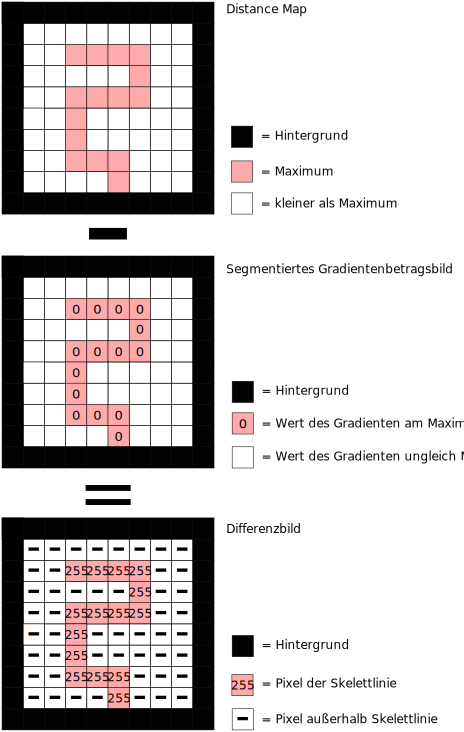
\includegraphics[width=1.0\linewidth]{./fig/skelettierung-prinzip}
%\caption{Die Idee der Skelettierung mittels Distanztransformation.}
%\label{fig:skelettierung-prinzip}
%\end{figure}
\subsection{Extracting Skeletons From Distance Maps}
\Autor{Sandra Schröder}\\\\ 
In dem Paper \emph{Extracting Skeletons from Distance Maps} beschreibt der Autor einen Algorithmus, der effizient und schnell
aus einem distanztransformierten Bild ein Skelett extrahiert \cite{extracting_skeletons_distancemaps}. Der Autor legt besonders hohen Wert darauf, dass die Extraktion keine komplizierten Berechnungen beinhaltet. Er möchte vor allem auf die Berechnung
von Ableitungen höherer Ordnung und die Auswertung von komplexen Gleichungen verzichten. Das Verfahren, welches der Autor zur 
Extraktion der Skelettlinien eines Objekt vorstellt, ist die sogenannte \emph{Ridge Point Detection} (deutsch: \emph{Gebirgskammdetektion}). Dabei nutzt der Autor eine grundlegende Eigenschaft der Distance Map. Wie in Abschnitt \ref{sec:distanztransformation} beschrieben, ist die Distance Map ein Grauwertgebirge, wobei der Gebirgskamm zentriert im Objekt liegt. Betrachtet man nur diesen Teil der Distance Map und projiziert ihn auf das Originalbild, 
lässt sich eine skelett-artige Beschreibung des Objekts erkennen.\\\\
Die Gebirgskammdetektion ist ein gradientenbasiertes Verfahren. Liegt ein Punkt auf den Gebirgskamm, so hat er in 
seiner unmittelbaren Umgebung den größten Abstand zum Objektrand und den größten Grauwert relativ zu seinen Nachbarn. Dieser Punkt ist somit ein lokales Maximum. Aufgrund dieser Tatsache eignet  sich der Gradient am besten, um solch einen Punkt zu detektieren. Der Gradient zeigt nach Definition in die Richtung des stärksten Anstiegs. Dies bedeutet, dass der Gradient eines Punktes, der nicht auf dem Kamm liegt, in die Richtung des Kammes zeigt. Wählt man nun Punkte näher am Kamm, so wird der Anstieg
geringer, da die Differenz zwischen dem Grauwert des betrachteten Gebirgspunktes und dem aktuell gewählten Punkt kleiner wird. Überquert man den Kamm, kehrt sich die Richtung des Gradienten um und zeigt wieder zum Kamm. Hier findet ein Vorzeichenwechsel des Gradientenbetrags statt. Der Punkt auf dem Gebirgskamm bildet eine \emph{sign barrier} zwischen den Gradientenbeträgen der sich gegenüberliegenden Punkte, wobei sich der Gebirgspunkt zwischen diesen beiden Punkten befindet. Diese
Beobachtung ist in Abbildung \ref{fig:paper_ridge_point_detection} dargestellt. Es ist ein Querschnitt eines Grauwertgebirges
abgebildet. Legt man nun eine Projektionslinie genau durch das lokale Maximum (roter Punkt), und projiziert die Gradienten (violette Pfeile) der sich gegenüberliegenden Punkte (blau) auf diese Linie, so kann man erkennen, dass die Projektionen der Gradienten (orangene Pfeile) genau in die entgegengesetzte Richtung zeigen.\
\begin{figure}
\centering
\includegraphics[width=1.0\linewidth]{./fig/paper_ridge_point_detection.pdf}
\caption{Ridge Point Detection. Der rote Punkt ist ein lokales Maximum auf dem Gebirgskamm. Die blauen Punkte liegen sich
gegenüber und umschließen den roten Punkt. Ihre auf die Projektionlinie projizierten Gradientenrichtungen zeigen in entgegengesetzte Richtungen. Der rote Punkt bildet somit eine \emph{sign barrier} für die beiden Richtungen.}
\label{fig:paper_ridge_point_detection}
\end{figure}
Die Idee des Algorithmus ist, Projektionslinien durch die Distance Map zu legen und das Verhalten der Gradientenbeträge
auf diesen Lininen zu beobachten. Der Autor hat festgestellt, dass sich dabei mehrere Muster von Vorzeichenwechsel der
Gradientenbeträge erkennen lassen. Diese Muster können dabei ein Indiz für einen Gebirgspunkt und somit für einen Punkt des Skeletts sein. \\
Dabei stellt sich die Frage, wieviele Richtungen mit diesen Linien untersucht werden sollen. Man kann beobachten, dass es
einen Vorzeichenwechsel in den Gradientenbeträgen gibt, wenn die Projektionslinie den Gebirgskamm schneidet. Dementsprechend 
gibt es keinen Vorzeichenwechsel, wenn die Projektionslinie parallel zum Kamm verläuft. Findet man also in einer Richtung
keinen Gebirgskamm, so muss einer in der orthogonalen Richtung liegen. Deshalb genügt es, zwei zueinander senkrechte Richtungen
zu untersuchen. Dabei wählt man die eine Richtung parallel zur x-Achse und die andere Richtung parallel zur y-Achse des untersuchten Bildes.
\begin{figure}
\centering
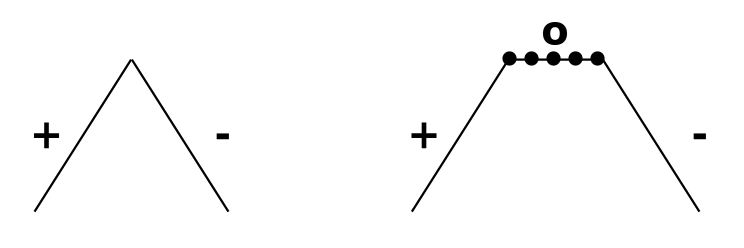
\includegraphics[width=0.8\linewidth]{./fig/muster_strong_good.pdf}
\caption{Muster für Hinweise auf einen Gebirgskamm. Diese beiden Muster sind ein starkes (\emph{strong}, linke Abbildung) und ein gutes (\emph{good}, rechte Abbildung) Indiz für einen Punkt auf dem Gebirgskamm. \textbf{TODO die Abbildung ist doof}}
\label{fig:muster_strong_good}
\end{figure}
Es existieren insgesamt vier Muster, die auf einen Gebirgskamm deuten. Zwei davon sind in Abbildung \ref{fig:muster_strong_good}
zu sehen. Die Muster beschreiben, in welcher Weise Vorzeichenwechsel zwischen zwei benachbarten Pixeln auftreten können. Die Symbole $+$ und $-$ die Richtungen der Gradienten. $+$ ist eine positive Richtung (bergauf), $-$ eine negative Richtung (bergab) auf einer Projektionslinie. Das Symbol $\circ$ besagt, dass sich in diesem Bereich der Gradient nicht ändert, da der Grauwert im nächsten Nachbarpunkt gleich ist. Die linke Abbildung entspricht genau der Beobachtung, wie sie anhand Abbildung
\ref{fig:paper_ridge_point_detection} beschrieben wurde. Schneidet die Projektionslinie genau einen Punkt auf dem Gebirgskamm,
erzeugt dieser Punkt einen Vorzeichwechsel zwischen den beiden Punkten, die den Punkt auf dem Kamm umschließen. Die rechte
Abbildung zeigt, dass es mehrere Punkte hintereinander in der Distance Map mit dem gleichen Grauwert geben kann, aber auch ein
Hinweis für einen Gebirgskamm sind. Dies entspricht im Grauwertgebirge einem Plateau.\\
Der Algorithmus sucht nun in x -und in y Richtung - von oben nach unten und von links nach rechts - in der Distance Map nach diesen Mustern und markiert die Punkte nach den Eigenschaften \emph{strong}, \emph{good}, \emph{weak} und \emph{none}. 
Diese Markierung gibt die Stärke der Sicherheit des Punktes wieder, ein Punkt auf dem Gebirgskamm zu sein. \\
Wurden alle Punkte in beide Richtungen untersucht, hat jeder Punkt ein passendes Label. Diese Labels werden weiter benutzt, um eine Graphenrepräsentation des Skeletts zu erstellen.\\
Der Algorithmus findet zu jedem Punkt das richtige Label und alle Punkte, die zu einem Gebirgskamm gehören \cite{extracting_skeletons_distancemaps}. Abbildung \ref{fig:paper_ergebnis} zeigt ein Ergebnis des Algorithmus. Die gestrichelte Linie in der rechten Abbildung beschreibt das theoretische Skelett, die grau unterlegten Punkte sind die vom Algorithmus gewählten Punkte, die zu einem Gebirgskamm gehören und einem Skelettpunkt entsprechen.
\begin{figure}
\centering
\includegraphics[width=0.7\linewidth]{./fig/paper_ergebnis}
\caption{Ergebnis der Ridge Point Detection \cite{extracting_skeletons_distancemaps}. Links: Graphische Darstellung. Rechts: Darstellung als Bildmatrix. }
\label{fig:paper_ergebnis}
\end{figure}
\section{Weitere Verfahren}
\Autor{Christopher Kroll}